\chapter{Potential outcome model}
\label{chapt:PotentialOM}

Il potential outcome model definisce l'effetto causale di un evento A come la differenza tra i due "stati" del mondo, cioè il mondo dove accade A e il mondo dove non accade A.

Poniamo ad esempio di voler capire se veramente un medicinale possa migliorare il mal di testa. Formalizziamo il problema ponendo X come l'insieme di covariate dei pazienti, D il regime di trattamento (che assume il valore 1 se viene dato il medicinale mentre assume valore 0 quando al paziente viene somministrato il placebo) e $Y^{obs}_i$ come il numero di minuti per cui persiste il mal di testa. 
Dunque se potessimo conoscere contemporaneamente  $Y^{obs}_i|D=1$ , che chiameremo $Y^{1}_i$, e $Y^{obs}_i|D=0$ , che chiameremo $Y^{0}_i$, allora calcolare se il medicinale causa un miglioramento risulterà molto semplice. Introduciamo un esempio numerico : 
\begin{table}[H]
\centering
\begin{tabular}{|c|c|c|c|c|}
\hline
Age & Sex & $Y^{0}_i$ & $Y^{1}_i$ & $\delta_i$ \\ \hline
20 & M & 20 & 21 & -1  \\ \hline
20 & F & 15 & 3 & 12 \\ \hline
20 & M & 8 & 10 & -2 \\ \hline
20 & F & 16 & 15 & 1 \\ \hline
30 & M & 12 & 13 & -1 \\ \hline
30 & F & 8 & 5 & 3 \\ \hline
30 & M & 2 & 11 & -9  \\ \hline
30 & F & 15 & 26 & 11 \\ \hline
\end{tabular}
\caption{Tabella esperimento }
\end{table}
Vediamo che il $\delta$ non è sempre positivo dunque la medicina non ha migliorato la situazione per tutti, notiamo però che in generale ha ridotto il tempo del malessere, questo però non basta, dobbiamo essere più precisi quantificando esattamente la tipologia e la dimensione dell'effetto.

\paragraph{Definizione parametri} \hspace{0pt} \\
\label{parag:param}
Definiamo quindi alcune quantità che ci risulteranno utili : 
\begin{itemize}
\item CATE o Conditional Average Treatment Effect è definito come $E[Y^{1}_i- Y^{0}_i|X] = E[\delta_i|X]$, quindi $CATE_{(M,20)}=E[\delta_i|X=(M,20)] \approx \frac{18-2}{2}=8$ , possiamo quindi dire che tra i maschi ventenni la medicina causa in media una riduzione di 8 minuti nella durata del mal di testa .
\item ATE o Average Treatment Effect è definito come  $E[Y^{1}_i- Y^{0}_i] = E[\delta_i]$, quindi $ATE= E[\delta_i] \approx \frac{18+12-2+18+3-9+11}{8}$.
\item ATT o Average Treatment on the Treated è definito come  $E[Y^{1}_i- Y^{0}_i|D=1] = E[\delta_i|D=1]$ 
\item ATU o Average Treatment on the Untreated è definito come 
$E[Y^{1}_i- Y^{0}_i|D=1] = E[\delta_i|D=0]$
\end{itemize}
 
Non possiamo calcolare gli ultimi due perché siamo ancora nel caso ipotetico dove conosciamo i due potential outcomes.
Ovviamente questa tabella non potrà mai essere riempita come abbiamo mostrato sopra perché possiamo veramente conoscere una sola quantità tra $Y^0_{i}$ e $Y^1_{i}$, sarà quindi impossibile avere certezza sulle quantità definite prima ma bisognerà stimarle. 
Dunque è utile fare la distinzione tra i valori \textit{fattuali} cioè cosa è veramente successo e \textit{controfattuale} cioè cosa sarebbe accaduto se il regime di trattamento fosse stato diverso.
Possiamo capire meglio la relazione tra potential outcome e observed outcome attraverso la  "switching equation": 
\begin{equation}
Y_i^{obs} = D_i \cdot Y^1_i + (1-D_i) \cdot Y^0_i
\label{eq:switching}
\end{equation}
Vediamo quindi che $Y_i^{obs} = Y^1_i$ quando $D_i =1$ ,mentre $Y_i^{obs} = Y^0_i$ quando $D_i = 0$. 
Bisogna precisare che la differenza tra $Y_i^{obs}$ e $Y^0_i,Y^1_i$ è che i primi sono valori effettivi, empirici che si possono osservare mentre gli ultimi sono valori ex-ante e dunque esistono prima che la $D_i$ venga somministrata.

Quello che invece ci ritroveremo nella realtà sarà una tabella più simile a questa 
\begin{table}[H]
\centering
\begin{tabular}{|c|c|c|c|}
\hline
Age & Sex & $Y^{0}_i$ & $Y^{1}_i$ \\ \hline
20 & M & 20 & ?  \\ \hline
20 & F & 15 & ? \\ \hline
20 & M & ? & 10 \\ \hline
20 & F & ? & 15  \\ \hline
30 & M & 12 & ? \\ \hline
30 & F & 8 & ? \\ \hline
30 & M & ? & 11   \\ \hline
30 & F & ? & 26 \\ \hline
\end{tabular}
\caption{Tabella esperimento }
\end{table}
Abbiamo dunque ridotto il problema della causalità ad un problema di \textit{Missing Data}, questa è la forza del modello usato.

\section{Studi randomizzati: Ruolo della randomizzazione}
Spesso si sente parlare di studi clinici randomizzati controllati, cioè studi in cui a metà dei partecipanti viene dato un placebo e all'altra metà il medicinale che è oggetto di studio, ovviamente né i medici né i pazienti sono a conoscenza di quali persone hanno assunto una o l'altra cosa. La situazione può essere espressa con un DAG in questa maniera: 
\begin{figure}[H]
\centering
	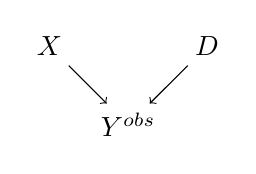
\begin{tikzpicture}
		\node (x) at (0,1) {$X$};
    		%\node (yz) at (0,0) {$Y^{1}$};
    		%\node (yo) at (2,0) {$Y^{0}$};
		\node (y) at (1,0) {$Y^{obs}$};
    		\node (D) at (2,1) {$D$};
    		%\path[->] (x) edge (yz);
    		%\path[->] (x) edge (yo);
    		\path[->] (x) edge (y);
    		%\path[<-] (T) edge (x);
    		\path[->] (D) edge (y);
	\end{tikzpicture}
\caption{Dag per studio randomizzato}
\label{fig:dag_random_EX}
\end{figure}
Ma perché questo procedimento è ormai la norma per verificare l'efficacia di un farmaco? E cosa ci può dire veramente un esperimento del genere? Sotto il potential outcome model questo procedimento può essere formalizzato tramite questa indipendenza
\begin{equation}
D \perp\!\!\!\perp (Y^{0},Y^{1})
\end{equation}
\label{eq:indipendence_r}

ciò significa che il trattamento non è amministrato in base ai potential outcome, ma in modo casuale. Non bisogna però confondersi e pensare che ciò implichi che $D \perp\!\!\!\perp Y^{obs}$, infatti ciò è espressamente falso ogni volta che il medicinale ha effetto su $Y^{obs}$.
Grazie all'equazione \ref{eq:indipendence_r} abbiamo che $E[Y^1_i] = E[Y^{1}_i | D_i = 1]  $ e la stessa cosa per $E[Y^0_i] = E[Y^{0}_i | D_i = 0] $.
Possiamo quindi dire che :
\begin{align}
ATE &= E[Y^1_i-Y^0_i ] \\ 
 &= E[Y^{1}_i | D_i = 1]- E[Y^{0}_i | D_i = 0]\label{eq:ATE_R} \\
	& =E[Y^{1}_i | D_i = 1]- E[Y^{0}_i | D_i = 1] \label{eq:ATT_R} \\
 &= E[Y^{1}_i | D_i = 0]- E[Y^{0}_i | D_i = 0] \label{eq:ATU_R}
  \end{align}

Nell'equazione \ref{eq:ATE_R} entrambi gli addenti sono quantità \textit{fattuali}, grazie alla legge dei grandi numeri stimiamo queste quantità con delle semplici medie, chiameremo quindi SDO la semplice differenza delle media osservate per i gruppi:
$$SDO = \frac{1}{N_1}\sum_i(y_i|d_i=1) - \frac{1}{N_2}\sum_i(y_i|d_i=0) \overset{\underset{\mathrm{(N_1, N_2) \rightarrow \infty}}{}}{=} ATE$$

Dall'equazione \ref{eq:ATT_R} e \ref{eq:ATU_R} possiamo concludere che nel caso randomizzato avremo che $ATE = ATT = ATU$.


\section{Studi osservazionali (?)} % esiste il termine?
Gli studi osservazionali (?) sono invece strutturati in modo diverso, i ricercatori osservano e raccolgono dati su individui o gruppi senza intervenire o manipolare alcun aspetto dell'ambiente di studio, per 2 motivi principali:
\begin{enumerate}
\item Potrebbe essere non etico o pratico dividere la popolazione in maniera casuale (immaginiamo di volere studiare se fumare causa un aumento nel rischio del cancro)
\item Gli eventi sono già accaduti (immaginiamo di volere studiare se i tassi di interesse incidano sul consumo)
\end{enumerate}

Dunque la cosa principale che cambia dal caso precedente è che $D \not \perp\!\!\!\perp (Y^{0},Y^{1})$, possiamo dunque rappresentare la situazione con il seguente DAG:
\begin{figure}[!h]
\centering
	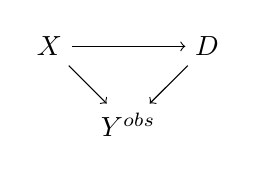
\begin{tikzpicture}
		\node (x) at (0,1) {$X$};
    		%\node (yz) at (0,0) {$Y^{1}$};
    		%\node (yo) at (2,0) {$Y^{0}$};
    		\node (y) at (1,0) {$Y^{obs}$};
    		\node (D) at (2,1) {$D$};
    		%\path[->] (x) edge (yz);
    		%\path[->] (x) edge (yo);
    		\path[->] (x) edge (D);
    		\path[->] (x) edge (y);
    		\path[->] (D) edge (y);
    		%\path[<-] (T) edge (x);
    		%\path[->] (T) edge (y);
	\end{tikzpicture}
\caption{Dag per studio osservazionale}
\label{fig:dag_OBS}
\end{figure}